\section{K-Means}
The principle of K-means is to select random centers for clusters, split the data set according to these centers and move them until they reach centers of density (see Algorithm \ref{kmean}). This method requires a desired number of clusters.

\begin{figure}[h!]
\fbox{
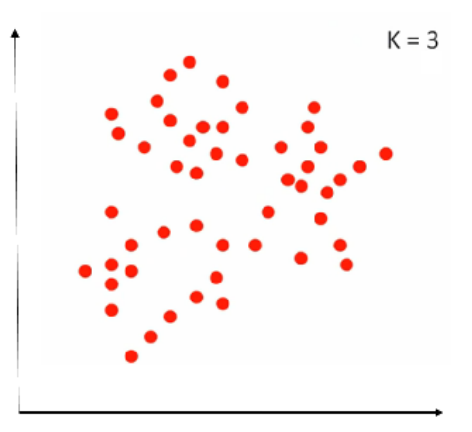
\includegraphics[width=0.3\textwidth, height=5.5cm]{Image/algo-kmeans1.png}
}
\fbox{
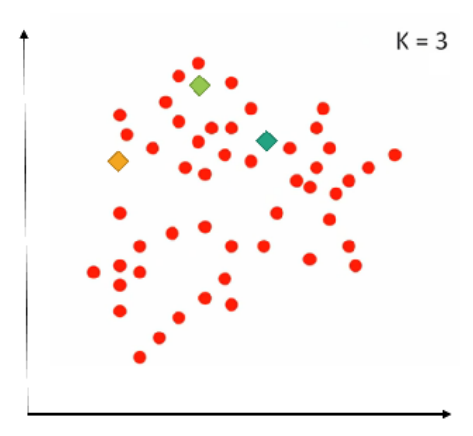
\includegraphics[width=0.3\textwidth, height=5.5cm]{Image/algo-kmeans2.png}
}
\fbox{
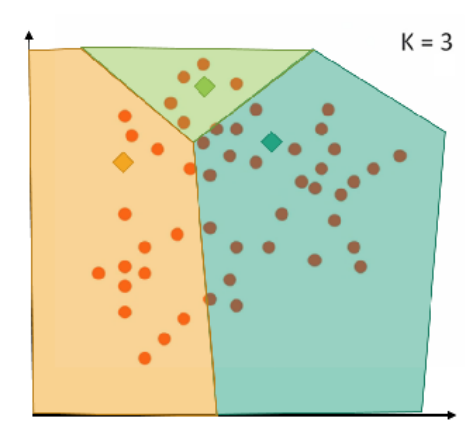
\includegraphics[width=0.3\textwidth, height=5.5cm]{Image/algo-kmeans3.png}
}
\begin{center}
\fbox{
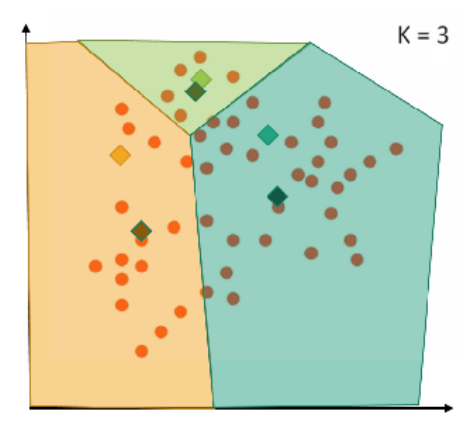
\includegraphics[width=0.3\textwidth, height=5.5cm]{Image/algo-kmeans4.png}
}
\fbox{
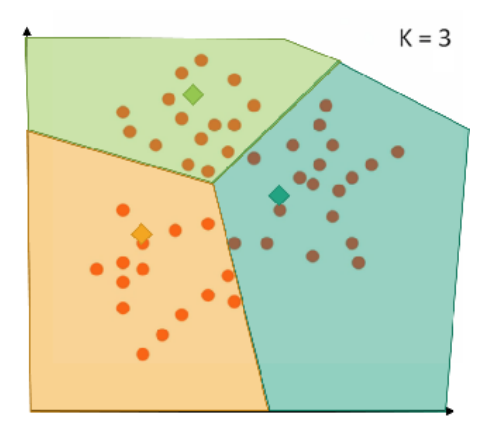
\includegraphics[width=0.3\textwidth, height=5.5cm]{Image/algo-kmeans5.png}
}
\end{center}
\caption{K-Mean algorithm - From right to left and top to bottom: Initial data, Select random centers, Split the data, Compute means, Move centers}
\end{figure}
\begin{algorithm}
\caption{K-Mean algorithm: returns cluster centers}
\label{kmean}
\begin{algorithmic}
\Loop
\State Split the data by matching each point to the closer cluster center
\State Compute the mean of each cluster
\If{The means and the centers are close}
\State \Return the means
\EndIf
\State Assign mean values to cluster centers 
\EndLoop
\end{algorithmic}
\end{algorithm}

However, this method is limited as we can only separated the clusters with hyperplanes, that does not work for non-linear separations (see Figure \ref{sepa}). To handle such cases, we pre-process the data by using kernel functions.
\begin{figure}
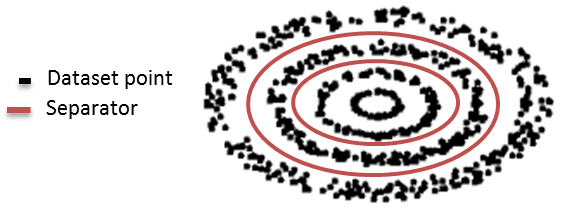
\includegraphics[width=0.6\textwidth]{Image/algo-sepa.png}\centering
\caption{Example of non linear separation\label{sepa}}
\end{figure}
\section{Kernel functions}
The main idea of the Kernel K-Mean algorithm is to map the data points into a higher dimensional space in order to lighten non linear separators (see Figure \ref{kern}). For this purpose, we pass the dataset ($x_1,...,x_n$) through a Kernel function that computes affinity between point using different approaches from simply finding the shortest distances:\\
\begin{equation}
\textbf{Polynomial Kernel }K(x_i,x_j) = (x_i^Tx_j + \gamma)^{\delta}
\end{equation}
\begin{equation}
\textbf{Exponential Kernel }K(x_i,x_j) = exp(-\frac{\Vert x_i-x_j\Vert^2}{2\sigma^2})
\end{equation}
\begin{equation}
\textbf{Sigmoïd Kernel }K(x_i,x_j) = tanh(\gamma (x_i^Tx_j) + \theta)
\end{equation}

The challenge of the Kernel K-Means algorithm is to select the right Kernel and adjust the parameters $\gamma$, $\delta$, $\sigma$ and $\theta$ in order to have the right space. Unfortunately, there is no known computation to find the perfect ones. It exists some methods to find interval that contains the optimal solution for the exponential Kernel but most of the time, the parameters are chosen empirically. That is why we offer the possibility to the user to select value for these parameters.
\begin{figure}[h!]
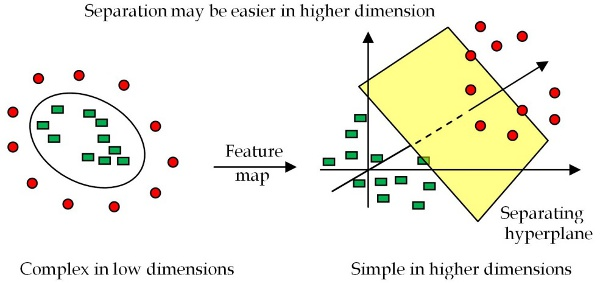
\includegraphics[width=0.6\textwidth]{Image/algo-kern.png}\centering
\caption{Projection on a higher dimensional space\label{kern}}
\end{figure}
